% ===== Page 1 =====
\section{Fields and Vector Spaces}\label{sec:fields-vs}\origpage{1}
\syllabusweek{Weeks 1--2 --- algebraic structures, fields, vector spaces, subspaces, linear independence, basis}

\subsection{Fields}\label{ss:fields}

\begin{definition}
A \term{field} is a set $\F$ together with two mappings called \term{addition} and \term{multiplication} shown as:
\[
\left.\begin{aligned}
\oplus &: \F\times\F\to\F\\
\odot &: \F\times\F\to\F
\end{aligned}\right\}\quad \text{$\F$ should be closed on both $\oplus$ and $\odot$.}
\]
\end{definition}

$\oplus$ and $\odot$ have the following properties (axioms):

\paragraph{Addition.}
\begin{enumerate}[label=(A\arabic*),leftmargin=3.2em]
\item $a\oplus b = b\oplus a \quad \forall a,b\in\F$ \hfill (commutativity)
\item $a\oplus(b\oplus c) = (a\oplus b)\oplus c \quad \forall a,b,c\in\F$ \hfill (associativity)
\item $\exists$ (there exists) $\0\in\F$ such that $a\oplus \0 = a \quad \forall a\in\F$ \hfill (additive identity)
\item For each $a\in\F$, $\exists\,{-a}\in\F$ such that $a\oplus(-a) = \0$ \hfill (additive inverse)
\end{enumerate}

\paragraph{Multiplication.}
\begin{enumerate}[label=(M\arabic*),leftmargin=3.2em]
\item $a\odot b = b\odot a \quad \forall a,b\in\F$ \hfill (commutativity)
\item $a\odot(b\odot c) = (a\odot b)\odot c \quad \forall a,b,c\in\F$ \hfill (associativity)
\item $\exists\,\1\in\F$ such that $a\odot \1 = a \quad \forall a\in\F$ \hfill (multiplicative identity)
\item For each $a\in\F$, $a\neq \0$, $\exists\,a^{-1}\in\F$ such that $a\odot a^{-1} = \1$ \hfill (multiplicative inverse)
\end{enumerate}

\paragraph{Distributivity.} The operations $\oplus$ \& $\odot$ satisfy
\begin{enumerate}[label=(D),leftmargin=3.2em]
\item $a\odot(b\oplus c) = (a\odot b)\oplus(a\odot c) \quad \forall a,b,c\in\F$ \hfill (distributivity)
\end{enumerate}

\begin{example}
$\F=\{0,1\}$ with $\oplus = +$ and $\odot = \cdot$\,.
\[ \oplus: \F\times\F\to\F, \qquad 1+1=2\notin\F \ \Rightarrow\ \text{not closed under } \oplus \]
Also no additive inverse exists for $1$ (A4): $1+a=0$ has no solution $a\in\{0,1\}$ (we would need $a=-1\notin\F$).
\begin{insight}[Remark]
With arithmetic \emph{modulo 2} ($1\oplus1=0$, $\odot$ the ordinary product) the set $\{0,1\}$ \emph{is} a field, usually denoted $\mathrm{GF}(2)$ or $\Z_2$: here $-1=1$ and $1^{-1}=1$. So whether a set is a field depends on the operations, not only on the set.
\end{insight}
\end{example}

\begin{example}
Set of real numbers $\R$ with the standard addition \& multiplication.
\[ \F=\R, \qquad \oplus = +, \qquad \odot=\cdot \qquad \Rightarrow \text{ A field} \]
\end{example}

% ===== Page 2 =====
\begin{example}
Let\origpage{2} $\F=\R\times\R=\R^2$ with $x = (x_1,x_2)\in\F$, $y = (y_1,y_2)\in\F$ and
\begin{align*}
x\oplus y &= (x_1+y_1,\; x_2+y_2)\\
x\odot y &= (x_1y_1-x_2y_2,\; x_2y_1+x_1y_2)
\end{align*}
\explain{Go over all axioms and check whether they are satisfied.}
Additive identity and inverse:
\begin{align*}
\0 &= (0,0)\\
-(x_1,x_2) &= (-x_1,-x_2)
\end{align*}
Assume as example (complex-number notation):
\begin{align*}
(x_1,x_2) &= x_1+jx_2\\
(y_1,y_2) &= y_1+jy_2\\[2pt]
x\oplus y &= x_1+y_1+j(x_2+y_2)\\
x\odot y &= x_1y_1-x_2y_2+j(x_2y_1+x_1y_2)
\end{align*}
% corrected: notes had x \oplus y = x_1+y_1+j(y_1+y_2); the second component of x\oplus y is x_2+y_2
\explain{The multiplication rule is exactly complex multiplication: $(x_1+jx_2)(y_1+jy_2) = x_1y_1-x_2y_2+j(x_2y_1+x_1y_2)$ since $j^2=-1$.}
Multiplicative identity and inverse:
\begin{align*}
\1 &= (1,0)\\
(x_1,x_2)^{-1} &= \left(\frac{x_1}{x_1^2+x_2^2},\; \frac{-x_2}{x_1^2+x_2^2}\right),
\qquad \frac{1}{x_1+jx_2} = \frac{x_1-jx_2}{x_1^2+x_2^2}
\end{align*}
$\therefore$ \key{This is a field.}
\begin{insight}
Check: $(x_1,x_2)\odot(x_1,x_2)^{-1} = \left(\frac{x_1^2+x_2^2}{x_1^2+x_2^2},\ \frac{x_2x_1-x_1x_2}{x_1^2+x_2^2}\right) = (1,0)=\1$, defined for every $x\neq\0=(0,0)$. The remaining axioms (commutativity, associativity, distributivity) are inherited from those of complex numbers; this field is simply $\C$ written as pairs of reals.
\end{insight}
\end{example}

\begin{example}
Let $\F=\R$ with $x\oplus y = xy$ and $x\odot y = x+y$. Is $\F$ a field?
\begin{align*}
x\oplus y &= xy = yx = y\oplus x \quad \forall x,y\in\F && \text{(A1)}\ \checkmark\\
x\oplus(y\oplus z) &= x(yz) = (xy)z = (x\oplus y)\oplus z \quad \forall x,y,z\in\F && \text{(A2)}\ \checkmark
\end{align*}
\paragraph{Identities and inverses.}
\begin{align*}
\0 &= 1: && 0\oplus a = \0 \ \Rightarrow\ \text{not satisfied } (0\cdot a = 1 \ \times)\\
\1 &= 0: && a\in\F \Rightarrow a^{-1} = -a
\end{align*}
\explain{The additive identity must satisfy $a\oplus\0=a\cdot\0=a$ for all $a$, so $\0=1$. Then the element $0$ has no additive inverse, since $0\oplus a=0\cdot a=0\neq1$ for every $a$ (A4 fails). Likewise $\1=0$ (as $a+0=a$), and $a\odot(-a)=0=\1$, so (M4) holds.}
\paragraph{Distributivity.}
\begin{align*}
x\odot(y\oplus z) &\overset{?}{=} (x\odot y)\oplus(x\odot z)\\
x+yz &\neq (x+y)(x+z) = x^2+xz+xy+yz \quad\text{(in general; e.g.\ $x=y=z=1$: $2\neq4$)}
\end{align*}
$\therefore$ \key{Not a field, as (A4) \& (D) fail.}
\end{example}

\begin{example}
$\R^{2\times2}$ with standard matrix addition \& multiplication: in general $AB\neq BA$, i.e.\ there is no multiplicative commutativity (M1).
\[
\R^n:\quad
\begin{cases}
n=1,2 & \Rightarrow \text{a field can be defined}\\
n=3,4,\dots & \Rightarrow \text{no field can be defined.}
\end{cases}
\]
\begin{insight}[Precise meaning]
Here ``define a field on $\R^n$'' means: componentwise addition and a multiplication that is compatible with real scaling (bilinear), so that $\R\subset\F$ sits inside as $(a,0,\dots,0)$. For $n=1$ we get $\R$, for $n=2$ we get $\C$ (previous example). For $n\ge3$ no such field exists (Frobenius/Hopf); e.g.\ for $n=4$ the quaternions satisfy every axiom except commutativity (M1), exactly like $\R^{2\times2}$ fails (M1) (and in addition (M4), as singular matrices have no inverse).
\end{insight}
\end{example}

% ===== Page 3 =====
\subsection{Vector Spaces}\label{ss:vector-spaces}

\begin{definition}
A\origpage{3} \term{linear space} (\term{vector space}) $\V$ is a set whose elements are called \term{vectors}, associated with a field $\F$ whose elements are called \term{scalars} and two operations $(\V,\F)$: addition $\oplus_{\V}$ and scalar multiplication $\odot_{\V}$ (the subscript is dropped when no confusion arises).
\[
\left.\begin{aligned}
\oplus &: \V\times\V\to\V\\
\odot &: \F\times\V\to\V
\end{aligned}\right\}\quad \text{$\V$ should be closed on addition \& multiplication (closedness)}
\]
\end{definition}

The following axioms should hold for $\oplus$ and $\odot$:

\paragraph{Addition.}
\begin{enumerate}[label=(A\arabic*),leftmargin=3.2em]
\item $x\oplus y = y\oplus x \quad \forall x,y\in\V$ \hfill (commutativity)
\item $x\oplus(y\oplus z) = (x\oplus y)\oplus z \quad \forall x,y,z\in\V$ \hfill (associativity)
\item $\exists\, 0_{\V}\in\V$ such that $x\oplus 0_{\V} = x \quad \forall x\in\V$ \hfill (additive identity)
\item For every $x\in\V$, $\exists\, {-x}\in\V$ such that $x\oplus(-x) = 0_{\V}$ \hfill (additive inverse)
\end{enumerate}

\needspace{9\baselineskip}
\paragraph{Scalar multiplication.}
\begin{enumerate}[label=(SM\arabic*),leftmargin=3.8em]
\item $a\odot_{\V}(b\odot_{\V} x) = (a\odot_{\F} b)\odot_{\V} x \quad \forall \underbrace{a,b\in\F}_{\text{scalars}} \quad \forall \underbrace{x\in\V}_{\text{vector}}$ \hfill (associativity)
\item $a\odot(x\oplus y) = (a\odot x)\oplus(a\odot y) \quad \forall a\in\F \quad \forall x,y\in\V$ \hfill (distributivity over $\oplus_{\V}$)
\item $(a\oplus_{\F} b)\odot x = (a\odot x)\oplus(b\odot x) \quad \forall a,b\in\F \quad \forall x\in\V$ \hfill (distributivity over $\oplus_{\F}$)
\item $\1\odot x = x \quad \forall x\in\V$, where $\1$ is the multiplicative identity of $\F$ \hfill (identity)
\end{enumerate}

\begin{example}
Prove $\0\odot x = 0_{\V} \quad \forall x\in\V$.

Let $y \triangleq \0\odot x$; then $y\in\V$ (as multiplication is closed).
\begin{align*}
y\oplus y &= (\0\odot x)\oplus(\0\odot x)\\
&\overset{\text{(SM3)}}{=} (\0\oplus\0)\odot x\\
&\overset{\text{(A3) of }\F}{=} \0\odot x = y
\end{align*}
% corrected: notes had "=>" between the members of this chain; they are equalities
\explain{(SM3) read from right to left; then $\0\oplus\0=\0$ is (A3) of the field $\F$.}
$\Rightarrow\ y\oplus y = y$ is proven.
\begin{align*}
\text{(A4)} &\Rightarrow \exists\, {-y} \text{ such that } y\oplus(-y) = 0_{\V}\\
\text{add $-y$ to both sides of } y\oplus y=y &\Rightarrow (y\oplus y)\oplus(-y) = y\oplus(-y)\\
\text{(A1), (A2)} &\Rightarrow (y\oplus(-y))\oplus y = y\oplus(-y)\\
\text{(A4)} &\Rightarrow y\oplus 0_{\V} = 0_{\V}\\
\text{(A3)} &\Rightarrow \underline{y = 0_{\V}}
\end{align*}
\begin{insight}
Since $y=\0\odot x$, this proves $\0\odot x=0_{\V}$. The same trick ($y\oplus y=y\Rightarrow y=0_{\V}$) also gives $a\odot 0_{\V}=0_{\V}$ for every $a\in\F$, and with (SM3) one gets $(-\1)\odot x = -x$, because $x\oplus((-\1)\odot x) = (\1\oplus(-\1))\odot x = \0\odot x = 0_{\V}$.
\end{insight}
\end{example}

% ===== Page 4 =====
\begin{example}
Linear\origpage{4} space $(\overset{\V}{\F^n},\overset{\F}{\F})$; i.e., the vector space of $n$ tuples in $\F$ over the field $\F$.
\[
x = (x_1,x_2,\dots,x_n), \qquad y = (y_1,y_2,\dots,y_n), \qquad \text{where } x_i,y_i\in\F\ \forall i
\]
Addition and scalar multiplication:
\begin{align*}
x\oplus_{\V} y &= (x_1\oplus_{\F} y_1,\; x_2\oplus_{\F} y_2,\;\dots,\; x_n\oplus_{\F} y_n)\\
a\odot_{\V} y &= (a\odot_{\F} y_1,\; a\odot_{\F} y_2,\;\dots,\; a\odot_{\F} y_n)
\end{align*}
\[
(\R^n,\R)\ \checkmark \qquad (\C^n,\R)\ \checkmark \qquad (\C^n,\C)\ \checkmark \qquad (\R^n,\C)\ \times
\]
\explain{$(\C^n,\R)$: a real multiple of a complex vector is still complex, so it is a vector space (of dimension $2n$ over $\R$).}
\explain{$(\R^n,\C)$: closure under scalar multiplication is violated: multiplying a real vector by a complex scalar gives a complex vector, which is $\notin\V$.}
\end{example}

\begin{example}
Set of all real valued functions $t\mapsto f(t)$ defined over the real line.
\begin{align*}
\F &= \R\\
\V &= \text{real valued functions}\\
(f\oplus_{\V} g)(t) &= f(t)\oplus_{\F} g(t)\\
(a\odot_{\V} f)(t) &= a\odot_{\F} f(t)
\end{align*}
\end{example}

\needspace{10\baselineskip}
\begin{example}
Set of all polynomials with degree $n=2$
\[ \V = \{a_0t^2+a_1t+a_2 \mid a_0,a_1,a_2\in\R \ \&\ a_0\neq0\} \]
$\oplus$ and $\odot$ are standard polynomial addition and scalar multiplication.

$\therefore$ Not a vector space!
\begin{align*}
P_1(t) &= t^2+2t+3 \in\V\\
P_2(t) &= -t^2+2t+3 \in\V\\
(P_1\oplus P_2)(t) &= 4t+6\notin\V
\end{align*}
\end{example}

\begin{example}
Set of all polynomials with degree $n\le2$ is a vector space.
\[ \V = \{a_0t^2+a_1t+a_2 \mid a_0,a_1,a_2\in\R\} \]
\end{example}

\subsection{Subspaces}\label{ss:subspaces}
\begin{definition}
Let $\V$ be a vector space over the field $\F$. A subset $\W$ of $\V$ is a \term{subspace} of $\V$ if and only if $(\W,\F)$ is itself a vector space.
\end{definition}
\begin{center}

\begin{tikzpicture}[baseline=(c.center)]
\draw (0,0) circle (0.6); \draw (0,-0.1) circle (0.32);
\node at (0.72,0.55) {\small$\V$}; \node at (0,-0.1) {\scriptsize$\W$};
\node (c) at (0,0) {};
\end{tikzpicture}
\qquad
$\left[\;\text{only show that}\quad \left.\begin{aligned}\oplus&: \V\times\V\to\V\\ \odot&: \F\times\V\to\V\end{aligned}\right\}\ \text{holds}\;\right]$
\end{center}

\begin{remark}
We can check whether a (nonempty) subset $\W$ is a subspace or not by checking \key{only closure under addition and scalar multiplication}:
\begin{align*}
&\text{(S1)} \quad w_1\oplus w_2\in\W && \forall w_1,w_2\in\W && \text{(closure under addition)}\\
&\text{(S2)} \quad a\odot w_1\in\W && \forall w_1\in\W,\ \forall a\in\F && \text{(closure under scalar multiplication)}
\end{align*}
\end{remark}
\begin{insight}[Why closure is enough]
All axioms that are identities ((A1), (A2), (SM1)--(SM4)) hold in $\W$ automatically because they hold in the bigger set $\V$. The two existence axioms follow from (S2): taking $a=\0$ gives $\0\odot w=0_{\V}\in\W$ (A3), and taking $a=-\1$ gives $(-\1)\odot w=-w\in\W$ (A4). In particular, \key{every subspace contains $0_{\V}$}; a quick test is: if $0_{\V}\notin\W$, then $\W$ is not a subspace.
\end{insight}

% ===== Page 5 =====
\begin{example}
$\V=\R^2$,\origpage{5} $\F=\R$, \quad $\W = \left\{ \bmat{a\\0} \;\middle|\; a\in\R \right\}$
\begin{align*}
w_1\in\W:&\quad w_1 = \bmat{a\\0} & w_1\oplus w_2 &= \bmat{a+b\\0}\in\W\\
w_2\in\W:&\quad w_2 = \bmat{b\\0} & c\odot w_1 &= \bmat{ca\\0}\in\W
\end{align*}
$\therefore$ $\W$ is a subspace of $\V$.
\end{example}

\needspace{10\baselineskip}
\begin{example}
$\V=\R^2$, $\F=\R$, \quad $\W = \left\{ \bmat{a\\1} \;\middle|\; a\in\R \right\}$
\[
w_1 = \bmat{a\\1}, \quad w_2=\bmat{b\\1} \qquad\Rightarrow\qquad w_1\oplus w_2 = \bmat{a+b\\2}\notin\W
\]
Not closed under vector addition or scalar multiplication (e.g.\ $0\odot w_1 = (0,0)\T\notin\W$: $\W$ does not contain the zero vector).

$\therefore$ $\W$ is \underline{not} a subspace.
\end{example}

\sep
$\blacktriangleright$ $\{0_{\V}\}$: zero dimensional vector space $\Rightarrow$ subspace.

\begin{center}
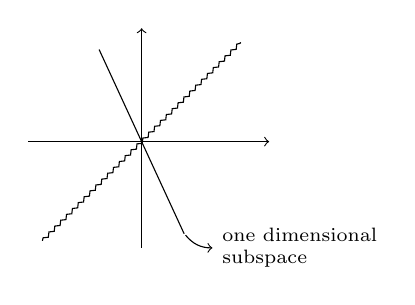
\begin{tikzpicture}[scale=0.9,baseline=(o.base)]
\coordinate (o) at (0,0);
\draw[->] (-1.6,0) -- (1.8,0);
\draw[->] (0,-1.5) -- (0,1.6);
% a line through the origin (steep, negative slope)
\draw (-0.6,1.3) -- (0.6,-1.3);
% one dimensional subspace: wavy line through the origin
\draw[decorate,decoration={snake,amplitude=0.6pt,segment length=3pt}] (-1.4,-1.4) -- (1.4,1.4);
\draw[->] (0.62,-1.32) to[bend right=25] (1.0,-1.5) node[right,align=left,font=\scriptsize] {one dimensional\\subspace};
\end{tikzpicture}
\qquad
$\begin{aligned}
\bmat{1\\1}&\in\W\\
-\bmat{1\\1}&\in\W
\end{aligned}
\qquad
a\odot x = 0_{\V} \ \text{ with } a=\0$
\end{center}
\explain{E.g.\ the line $\W=\Span\{(1,1)\T\}$ (the line $x_2=x_1$): with $(1,1)\T$ it also contains $-(1,1)\T$, and $\0\odot x=0_{\V}$ must lie in $\W$.}
\begin{itemize}[label=$\Rightarrow$,nosep]
\item \key{All subspaces should cross origin.}
\item For two dimensional subspace, include all $\R^2$.
\end{itemize}
\begin{insight}[Subspaces of $\R^2$]
The subspaces of $\R^2$ are exactly: $\{0_{\V}\}$ (dimension 0), every line through the origin (dimension 1), and $\R^2$ itself (dimension 2). A line not passing through the origin (such as $\{[a,\,1]\T\}$ above) is never a subspace.
\end{insight}

\begin{example}
$\V=\R^{2\times2}$, $\F=\R$, \quad $\W = \{\text{set of $2\times2$ real valued symmetric matrices}\}$
\begin{align*}
\bmat{a_1&b_1\\b_1&c_1}\oplus\bmat{a_2&b_2\\b_2&c_2} &= \bmat{a_1+a_2 & b_1+b_2\\ b_1+b_2 & c_1+c_2}\in\W\\
\alpha\bmat{a_1&b_1\\b_1&c_1} &= \bmat{\alpha a_1&\alpha b_1\\ \alpha b_1&\alpha c_1}\in\W
\end{align*}
$\therefore$ $\W$ is a subspace of $\V$.
\end{example}

\begin{example}
\begin{tabular}[t]{@{}l@{\ }l}
$\V$: & set of real valued functions defined over $\R$\\
$\W_1$: & set of real valued continuous functions\\
$\W_2$: & set of all real valued functions which are discontinuous at $t=1$
\end{tabular}

\needspace{11\baselineskip}
$\therefore$ $\W_1$ is a subspace. For $\W_2$:
\begin{center}
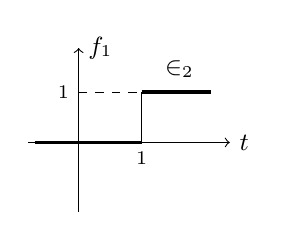
\begin{tikzpicture}[scale=0.8]
% f1: 0 for t<1, 1 for t>1
\draw[->] (-0.8,0) -- (2.4,0) node[right] {\small$t$};
\draw[->] (0,-1.1) -- (0,1.5) node[right] {\small$f_1$};
\draw[very thick] (-0.7,0) -- (1,0);
\draw[very thick] (1,0.8) -- (2.1,0.8);
\draw[thin] (1,0) -- (1,0.8);
\draw[dashed] (0,0.8) -- (1,0.8);
\node[left] at (0,0.8) {\scriptsize 1};
\node[below] at (1,0) {\scriptsize 1};
\node[below] at (1.6,1.45) {\small$\in\W_2$};
\end{tikzpicture}
\quad
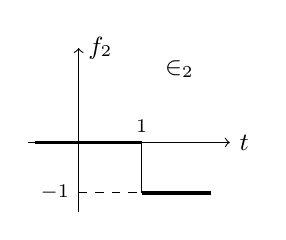
\begin{tikzpicture}[scale=0.8]
% f2: 0 for t<1, -1 for t>1
\draw[->] (-0.8,0) -- (2.4,0) node[right] {\small$t$};
\draw[->] (0,-1.1) -- (0,1.5) node[right] {\small$f_2$};
\draw[very thick] (-0.7,0) -- (1,0);
\draw[very thick] (1,-0.8) -- (2.1,-0.8);
\draw[thin] (1,0) -- (1,-0.8);
\draw[dashed] (0,-0.8) -- (1,-0.8);
\node[left] at (0,-0.8) {\scriptsize $-1$};
\node[above] at (1,0) {\scriptsize 1};
\node[below] at (1.6,1.45) {\small$\in\W_2$};
\end{tikzpicture}
\quad
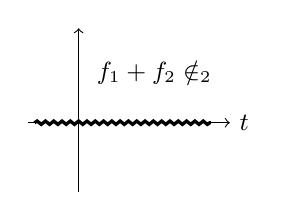
\begin{tikzpicture}[scale=0.8]
% f1+f2 = 0 (continuous)
\draw[->] (-0.8,0) -- (2.4,0) node[right] {\small$t$};
\draw[->] (0,-1.1) -- (0,1.5);
\draw[very thick,decorate,decoration={snake,amplitude=0.6pt,segment length=3pt}] (-0.7,0) -- (2.1,0);
\node at (1.2,0.8) {\small$f_1+f_2\notin\W_2$};
\end{tikzpicture}
\end{center}
% corrected: the middle graph is labeled "\in W" in the notes; it is meant as \in W_2
\explain{$f_1$ and $f_2$ both jump at $t=1$, but $f_1+f_2$ is the zero function, which is continuous.}
$\therefore$ Not closed under vector addition \& scalar multiplication (multiply with zero: $0\cdot f_1$ is the zero function, which is continuous, so $\notin\W_2$). Hence $\W_2$ is \underline{not} a subspace.
\begin{insight}
$\W_1$ is a subspace because sums and scalar multiples of continuous functions are continuous (and the zero function is continuous). $\W_2$ fails already the quick test: the zero vector of $\V$ (the zero function) is not in $\W_2$.
\end{insight}
\end{example}

% ===== Page 6 =====
\subsection{Sums, Intersections and Products of Subspaces}\label{ss:sums}
\begin{definition}
The\origpage{6} \term{sum} $Y+Z$ of two subsets $Y$ \& $Z$ of a linear space is the set of all vectors $y+z$ where $y\in Y$ and $z\in Z$.
\[ Y+Z \triangleq \{ y+z \mid y\in Y,\ z\in Z\} \]
\end{definition}

\begin{example}
$\V=\R^2$,
\[
Y = \left\{\bmat{a\\0} \;\middle|\; 2\le a\le3\right\}, \qquad
Z = \left\{\bmat{0\\b} \;\middle|\; 1\le b\le2\right\}
\]
\begin{center}
\begin{tikzpicture}[scale=0.8]
\draw[->] (-0.5,0) -- (4,0) node[below] {\small$y$};
\draw[->] (0,-1.2) -- (0,3) node[left] {\small$z$};
\fill[pattern=north east lines] (2,1) rectangle (3,2);
\draw (2,1) rectangle (3,2);
\node at (3.4,2.4) {\small$Y+Z$};
\draw[thick,decorate,decoration={snake,amplitude=0.7pt,segment length=3pt}] (0,1) -- (0,2);
\draw[thick,decorate,decoration={snake,amplitude=0.7pt,segment length=3pt}] (2,0) -- (3,0);
\draw[dashed] (0,1) -- (2,1); \draw[dashed] (0,2) -- (2,2);
\draw[dashed] (2,0) -- (2,1); \draw[dashed] (3,0) -- (3,1);
\draw[->] (0,0) -- (2.4,1.5);
\node[left] at (0,1) {\scriptsize1}; \node[left] at (0,2) {\scriptsize2};
\node[below] at (2,-0.1) {\scriptsize2}; \node[below] at (3,-0.1) {\scriptsize3};
\end{tikzpicture}
\end{center}
If instead $Y$ and $Z$ are two lines through the origin (subspaces), every vector $x$ can be decomposed as $x=y+z$ with $y\in Y$, $z\in Z$:
\begin{center}
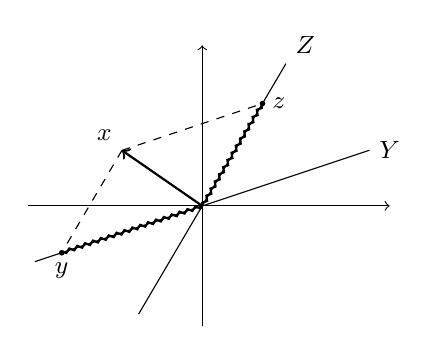
\begin{tikzpicture}[scale=0.85]
\draw[->] (-2.6,0) -- (2.8,0);
\draw[->] (0,-1.8) -- (0,2.4);
% Y: line through origin with slope 1/3, Z: line with slope 1.7
\draw (-2.5,-0.833) -- (2.5,0.833) node[right] {\small$Y$};
\draw (-0.95,-1.615) -- (1.25,2.125) node[above right] {\small$Z$};
% y in Y (negative direction), z in Z, x = y + z
\coordinate (y) at (-2.1,-0.7);
\coordinate (z) at (0.9,1.53);
\coordinate (x) at (-1.2,0.83);
\draw[thick,decorate,decoration={snake,amplitude=0.6pt,segment length=3pt}] (0,0) -- (y);
\draw[thick,decorate,decoration={snake,amplitude=0.6pt,segment length=3pt}] (0,0) -- (z);
\fill (y) circle (1.2pt) node[below] {\small$y$};
\fill (z) circle (1.2pt) node[right] {\small$z$};
\draw[->,thick] (0,0) -- (x) node[above left] {\small$x$};
\draw[dashed] (x) -- (z);
\draw[dashed] (x) -- (y);
\end{tikzpicture}
\end{center}
The same can be done for every vector, so $Y+Z = \R^2$ $\Rightarrow$ the sum of two subspaces is again a subspace.
\end{example}

\needspace{16\baselineskip}
\begin{remark}
If $Y$ \& $Z$ are both subspaces, then \key{$Y+Z$ is a subspace}.
\end{remark}
\begin{proof}
Let $x_1, x_2\in Y+Z$:
\begin{gather*}
x_1 = \underset{\in Y}{y_1}+\underset{\in Z}{z_1}, \qquad x_2 = \underset{\in Y}{y_2}+\underset{\in Z}{z_2}\\[6pt]
x_1+x_2 = y_1+z_1+y_2+z_2 = \underbrace{y_1+y_2}_{\in Y}+\underbrace{z_1+z_2}_{\in Z}
\end{gather*}
\explain{As $Y$ and $Z$ are subspaces, they are closed under addition.}
Similarly, for any scalar $\alpha$:
\[
\underbrace{\alpha x_1}_{\in Y+Z} = \alpha(y_1+z_1) = \underbrace{\alpha y_1}_{\in Y}+\underbrace{\alpha z_1}_{\in Z}
\]
Closed under scalar multiplication.

$\therefore$ $Y+Z$ is a subspace.
\end{proof}

\sep
For the two lines $Y$, $Z$ of the previous example:
\[ Y\cap Z = \left\{\bmat{0\\0}\right\} \text{ is a subspace} \Rightarrow \text{not a coincidence!} \]

\begin{remark}
If $Y$ \& $Z$ are subspaces, then \key{$Y\cap Z$ is a subspace}.

($Y\cup Z$ is closed under scalar multiplication but not closed under addition, which is the case in the previous example) $\Rightarrow$ \key{$Y\cup Z$ is not a subspace \underline{generally}}.
% corrected: notes had "Y u Z is not closed under addition but not closed under scalar multiplication"; Y u Z is always closed under scalar multiplication
\end{remark}
\begin{insight}
\emph{Proof for $Y\cap Z$:} if $x_1,x_2\in Y\cap Z$, then $x_1+x_2\in Y$ and $x_1+x_2\in Z$ (both are subspaces), so $x_1+x_2\in Y\cap Z$; similarly $\alpha x_1\in Y\cap Z$.

\emph{Why $Y\cup Z$ fails:} for the two lines, $y\in Y$, $z\in Z$ nonzero give $y+z$, which lies on neither line. In fact $Y\cup Z$ is a subspace only if $Y\subseteq Z$ or $Z\subseteq Y$. The sum $Y+Z$ is the \key{smallest subspace containing $Y\cup Z$}.
\end{insight}

\begin{definition}[Product space]
Let $(\V,\F)$ \& $(\W,\F)$ be two linear spaces defined over the same field $\F$. The \term{product} of $(\V,\F)$ \& $(\W,\F)$ is defined as:
\begin{align*}
\V\times\W &= \{(v,w) \mid v\in\V,\ w\in\W\}\\
(v_1,w_1)\oplus_{\V\times\W}(v_2,w_2) &= (v_1\oplus_{\V} v_2,\; w_1\oplus_{\W} w_2)\\
\alpha\odot_{\V\times\W}(v_1,w_1) &= (\alpha\odot_{\V} v_1,\; \alpha\odot_{\W} w_1)
\end{align*}
% corrected: notes had w_1 \oplus_V w_2 and \alpha \odot_V w_1; the second components use the operations of W
\[
\Rightarrow\quad
(\underset{\V\times\W}{\R^2},\underset{\F}{\R}) = (\underset{\V}{\R},\underset{\F}{\R})\times(\underset{\W}{\R},\underset{\F}{\R})
\]
\end{definition}
\explain{In general $\dim(\V\times\W)=\dim\V+\dim\W$; e.g.\ $\R^n\times\R^m=\R^{n+m}$.}

% ===== Page 7 =====
\subsection{Linear Combinations, Span and Linear Independence}\label{ss:span-li}
\begin{definition}
A\origpage{7} \term{linear combination} of $n$ vectors $x_1,x_2,\dots,x_n$ of a linear space $\V$ is a vector of the form
\[ a_1x_1+a_2x_2+\dots+a_nx_n = \sum_{i=1}^{n} a_ix_i \qquad \text{where } a_i\in\F \text{ for } i=1,\dots,n \]
The set of all linear combinations of $x_1,\dots,x_n$, i.e.
\[ \left\{ \sum_{i=1}^{n} a_ix_i \;\middle|\; a_i\in\F,\ i=1,\dots,n \right\} \]
is called the \term{span} of $\{x_1,\dots,x_n\}$, denoted $\Span\{x_1,\dots,x_n\}$.
\end{definition}

For $\V=\R^2$:
\begin{align*}
&x_1=\bmat{1\\0},\ x_2=\bmat{0\\1}: && a_1\bmat{1\\0}+a_2\bmat{0\\1} = \bmat{a_1\\a_2} &&\Rightarrow\ \Span\{x_1,x_2\}=\R^2\\
&x_1=\bmat{1\\0},\ x_2=\bmat{0\\1},\ x_3=\bmat{1\\1}: && && \Rightarrow\ \Span\{x_1,x_2,x_3\}=\R^2
\end{align*}
\explain{$x_3$ is redundant: $x_3=x_1+x_2$ is already a linear combination of $x_1,x_2$, so adding it does not enlarge the span.}

\begin{definition}
Vectors $x_1,\dots,x_n\in\V$ are said to be \term{linearly independent} if and only if
\[ a_1x_1+a_2x_2+\dots+a_nx_n = 0_{\V} \quad\text{implies}\quad a_1=a_2=\dots=a_n=\0 \]
If $\exists\, a_1,\dots,a_n$, not all equal to $\0$, such that
\[ a_1x_1+\dots+a_nx_n = 0_{\V}, \]
then $x_1,x_2,\dots,x_n$ are \term{linearly dependent}.
\end{definition}

\begin{example}
$x_1=\bmat{1\\0}$, $x_2=\bmat{0\\1}$:
\[
a_1\bmat{1\\0}+a_2\bmat{0\\1} = \bmat{0\\0} = \bmat{a_1\\a_2}
\quad\Rightarrow\quad a_1=a_2=0 \quad\Rightarrow\quad \text{linearly independent}
\]
\end{example}

\begin{example}
$x_1=\bmat{1\\0}$, $x_2=\bmat{0\\1}$, $x_3=\bmat{1\\1}$:
\[
a_1\bmat{1\\0}+a_2\bmat{0\\1}+a_3\bmat{1\\1} = \bmat{0\\0}
\ \Rightarrow\
\begin{aligned} a_1+a_3&=0\\ a_2+a_3&=0 \end{aligned}
\ \Rightarrow\
\text{e.g. } a_1=a_2=1,\ a_3=-1
\]
$\therefore$ linearly dependent.
\end{example}

\begin{example}
Consider the linear space of polynomials of degree $n\le2$, and
\[
P_1(t)=1, \quad P_2(t)=1+t, \quad P_3(t)=1+t+t^2, \qquad P=\{P_1(t),P_2(t),P_3(t)\}.
\]
Is $P$ linearly independent?
\begin{align*}
& a_1\cdot1+a_2(1+t)+a_3(1+t+t^2) = 0(t) && (\text{zero polynomial})\\
\Rightarrow\ & (a_1+a_2+a_3)+(a_2+a_3)t+a_3t^2 = 0(t) \ \Rightarrow\ a_1=a_2=a_3=0
\end{align*}
\explain{A polynomial is the zero polynomial only if all its coefficients vanish: $a_3=0$ (from $t^2$), then $a_2+a_3=0\Rightarrow a_2=0$ (from $t$), then $a_1+a_2+a_3=0\Rightarrow a_1=0$.}
$\therefore$ $P$ is linearly independent.
\end{example}

% ===== Page 8 =====
\needspace{12\baselineskip}
\begin{example}
$\V$:\origpage{8} set of all continuous functions defined over the real line.
\[ S = \left\{ \cos t,\ \sin t,\ \cos\!\left(t-\tfrac{\pi}{3}\right) \right\}. \quad \text{Is $S$ linearly independent?} \]
\[
a\cos t+b\sin t+c\,
\underbrace{\cos\!\left(t-\tfrac{\pi}{3}\right)}_{\cos t\,\cdot\,\cos\frac{\pi}{3}\;+\;\sin t\,\cdot\,\sin\frac{\pi}{3}} = 0(t)\quad \forall t,
\qquad \cos\tfrac{\pi}{3} = \tfrac12,\quad \sin\tfrac{\pi}{3} = \tfrac{\sqrt3}{2}
\]
Collecting terms:
\[ \left(a+\tfrac{c}{2}\right)\cos t+\left(b+\tfrac{\sqrt3}{2}c\right)\sin t = 0(t), \]
which holds for $a=-\tfrac{c}{2}$, $b=-\tfrac{\sqrt3}{2}c$ with any $c$. Choosing $a=-\tfrac12$, $b=-\tfrac{\sqrt3}{2}$, $c=1$ gives the zero function.

$\therefore$ \key{$S$ is \underline{not} linearly independent.}
\end{example}

\sep
Linear independence of the columns of a matrix $A = [c_1 \mid c_2 \mid \dots \mid c_n]$: consider $Ax=0$, i.e.
\[
[c_1 \mid c_2 \mid \dots \mid c_n]\bmat{x_1\\x_2\\\vdots\\x_n}
= \underbrace{c_1x_1+c_2x_2+\dots+c_nx_n}_{\text{zero}} = \bmat{0\\0\\\vdots\\0}
\]
\explain{$Ax$ is a linear combination of the columns of $A$ with coefficients $x_i$. Hence: \key{the columns $c_1,\dots,c_n$ are linearly independent $\iff$ $Ax=0$ has only the solution $x=0$}; any nonzero solution $x$ gives a dependence relation among the columns.}

\subsection{Basis, Dimension and Coordinates}\label{ss:basis}
\begin{definition}
Let $\V$ be a linear space and set of vectors $B=\{x_1,\dots,x_n\}$ be a subset of $\V$. $B$ is said to be a \term{basis} for $\V$ if and only if
\begin{enumerate}[label=(\roman*)]
\item $\Span B=\V$, and
\item $B$ is a linearly independent set.
\end{enumerate}
\end{definition}

For $\R^2$:
\begin{align*}
B_1 &= \left\{\bmat{1\\1}\right\} && \times\ \text{not a basis}\\
B_2 &= \left\{\bmat{1\\1},\bmat{1\\-1}\right\} && \checkmark\\
B_3 &= \left\{\bmat{1\\1},\bmat{1\\-1},\bmat{0\\1}\right\} && \times\ \text{not linearly independent}\\
B_4 &= \left\{\bmat{0\\1},\bmat{1\\0}\right\} && \checkmark\\
B_5 &= \left\{\bmat{1\\0},\bmat{1\\1}\right\} && \checkmark
\end{align*}
\explain{The two basis vectors should not be on the same line through the origin (their spans intersect only at the origin); there are infinitely many bases and the number of vectors is always 2.}
\explain{E.g.\ for $B_3$: $(0,1)\T=\tfrac12(1,1)\T-\tfrac12(1,-1)\T$. For $B_1$: $\Span B_1$ is only the line $x_2=x_1$, not $\R^2$.}

\begin{remark}
There are infinitely many basis sets for a linear space. \key{All of these basis sets have the same number of elements.} That number is called \term{dimension} of $\V$. If the dimension is finite, $\V$ is said to be \term{finite dimensional}. Otherwise, $\V$ is \term{infinite dimensional}.
\end{remark}

\begin{example}
$\V$ is the set of $2\times2$ real valued symmetric matrices:
\begin{gather*}
\bmat{a&b\\b&c} = a\bmat{1&0\\0&0}+b\bmat{0&1\\1&0}+c\bmat{0&0\\0&1}\\
B = \left\{ \bmat{1&0\\0&0},\bmat{0&1\\1&0},\bmat{0&0\\0&1} \right\}
\end{gather*}
\explain{3 elements (dimension 3).}
Infinite dimensional linear space $\Rightarrow$ set of continuous functions.
\explain{For every $n$, the functions $1,t,t^2,\dots,t^n$ are continuous and linearly independent, so no finite set can span this space.}
\end{example}

% ===== Page 9 =====
\begin{definition}
If\origpage{9} $y\in\V$ and $B=\{x_1,x_2,\dots,x_n\}$ is a basis set for $\V$, then there is a \key{unique} $n$-tuple of scalars $(a_1,a_2,\dots,a_n)$ such that
\[ y = \sum_{i=1}^{n} a_ix_i \]
The scalars $(a_1,a_2,\dots,a_n)$ are called \term{components} (\term{coordinates}), \term{representations} of $y$ with respect to (w.r.t.) basis $B$. We denote the representation of $y$ w.r.t.\ $B$ by $[y]_B$.
\end{definition}
With $B$ the basis of symmetric matrices above:
\[
y = \bmat{1&2\\2&3}\in\V, \qquad [y]_B = \underset{\substack{\uparrow\\\text{unique}}}{\bmat{1\\2\\3}}, \qquad y\in\V, \quad [y]_B\in\R^3
\]

$\blacktriangleright$ Why should representation be unique?
\begin{proof}
$[y]_B$ is unique. (Proof by contradiction)

Suppose $[y]_B$ is \underline{not} unique:
\[
[y]_B = \bmat{\alpha_1\\\alpha_2\\\vdots\\\alpha_n}, \qquad [y]_B = \bmat{\beta_1\\\beta_2\\\vdots\\\beta_n}, \qquad \exists\, i \text{ such that } \alpha_i\neq\beta_i
\]
By the representation definition,
\[
y = \sum_{i=1}^{n}\alpha_ix_i, \qquad y=\sum_{i=1}^{n}\beta_ix_i
\qquad\Rightarrow\qquad
0_{\V} = \sum_{i=1}^{n}(\alpha_i-\beta_i)x_i
\]
\explain{A linear combination of the basis vectors equal to zero with some of the coefficients nonzero, as $\alpha_i-\beta_i\neq0$.}
% corrected: notes had "some of the vectors are nonzero"; it is the coefficients alpha_i - beta_i that are nonzero
$\therefore$ $x_i$ are linearly dependent $\Rightarrow$ contradiction.
\end{proof}

\begin{example}
$\V = \Span\{\cos t,\sin t\}$, \quad $B = \{\cos t,\sin t\}$
\[
y \triangleq \cos\!\left(t-\tfrac{\pi}{3}\right) = \tfrac12\cos t+\tfrac{\sqrt3}{2}\sin t
\qquad\Rightarrow\qquad [y]_B = \bmat{1/2\\\sqrt3/2}
\]
\end{example}

\subsection{Change of Basis}\label{ss:change-basis}
\begin{theorem}[Change of basis]
Let $\V$ be an $n$-dimensional linear space over $\R$. Let $B_1$ and $B_2$ be two basis sets for $\V$. Then, there exists an $n\times n$ \key{real invertible matrix $P$} such that
\[ [v]_{B_1} = P\,[v]_{B_2} \quad \forall v\in\V \]
\end{theorem}
\begin{center}
\begin{minipage}{0.5\textwidth}
\begin{gather*}
B_1 = \left\{\bmat{1\\0},\bmat{0\\1}\right\}, \qquad B_2 = \left\{\bmat{1\\1},\bmat{1\\-1}\right\}\\[4pt]
v = \alpha_1\bmat{1\\0}+\alpha_2\bmat{0\\1}\\[4pt]
[v]_{B_1} = \bmat{\alpha_1\\\alpha_2}, \qquad
[v]_{B_2} = \bmat{\alpha_1'\\\alpha_2'}
\end{gather*}
\end{minipage}\hfill
\begin{minipage}{0.42\textwidth}
\centering
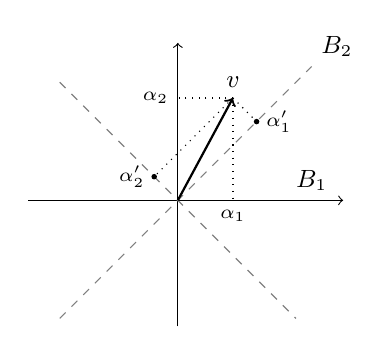
\begin{tikzpicture}[scale=1.0]
\draw[->] (-1.9,0) -- (2.1,0);
\draw[->] (0,-1.6) -- (0,2.0);
\node[above] at (1.7,0) {\small$B_1$};
% B_2 axes: y = x and y = -x
\draw[dashed,gray] (-1.5,-1.5) -- (1.7,1.7) node[above right,black] {\small$B_2$};
\draw[dashed,gray] (-1.5,1.5) -- (1.5,-1.5);
% v = (0.7,1.3) = 1.0*(1,1) - 0.3*(1,-1)
\draw[->,thick] (0,0) -- (0.7,1.3) node[above] {\small$v$};
\draw[dotted] (0.7,1.3) -- (0.7,0) node[below] {\scriptsize$\alpha_1$};
\draw[dotted] (0.7,1.3) -- (0,1.3) node[left] {\scriptsize$\alpha_2$};
\draw[dotted] (0.7,1.3) -- (1.0,1.0);
\draw[dotted] (0.7,1.3) -- (-0.3,0.3);
\fill (1.0,1.0) circle (1pt) node[right] {\scriptsize$\alpha_1'$};
\fill (-0.3,0.3) circle (1pt) node[left] {\scriptsize$\alpha_2'$};
\end{tikzpicture}
\end{minipage}
\end{center}
\begin{insight}[Finding $P$ for this example]
Write $v$ in terms of $B_2$:
\[ v=\alpha_1'\bmat{1\\1}+\alpha_2'\bmat{1\\-1}=\bmat{1&1\\1&-1}\bmat{\alpha_1'\\\alpha_2'}. \]
Since the $B_1$-coordinates are just the entries of $v$,
\[
[v]_{B_1}=\underbrace{\bmat{1&1\\1&-1}}_{P}[v]_{B_2},
\qquad
P^{-1}=\frac12\bmat{1&1\\1&-1}.
\]
In general, \key{the $j$-th column of $P$ is $[\,j\text{-th vector of }B_2\,]_{B_1}$}. $P$ is invertible because its columns are coordinates of a basis, hence linearly independent. For the drawn vector $v=(0.7,1.3)\T$: $[v]_{B_2}=P^{-1}[v]_{B_1}=(1,-0.3)\T$.
\end{insight}

\begin{example}
Consider $\V$: polynomials with degree $n\le2$.
\[
B_1 = \{\overset{v_1}{1},\ \overset{v_2}{1+t},\ \overset{v_3}{1+t+t^2}\},
\qquad
B_2 = \{\overset{w_1}{1},\ \overset{w_2}{t},\ \overset{w_3}{t^2}\}
\]
Find $P$ such that $[v]_{B_1} = P\,[v]_{B_2}$ $\forall v\in\V$.
% ===== Page 10 =====
\origpage{10}
\needspace{12\baselineskip}
\begin{align*}
v=w_1:&\quad [w_1]_{B_2} = \bmat{1\\0\\0} \Rightarrow P\bmat{1\\0\\0} = \text{1st column of } P = [w_1]_{B_1} = \bmat{1\\0\\0}\\
v=w_2:&\quad [w_2]_{B_2} = \bmat{0\\1\\0} \Rightarrow P\bmat{0\\1\\0} = \text{2nd column of } P = [w_2]_{B_1} = \bmat{-1\\1\\0}\\
v=w_3:&\quad [w_3]_{B_2} = \bmat{0\\0\\1} \Rightarrow P\bmat{0\\0\\1} = \text{3rd column of } P = [w_3]_{B_1} = \bmat{0\\-1\\1}
\end{align*}
% corrected: notes had "P = [w_1]_{B_1}", "P = [w_2]_{B_1}" (subscript hard to read) and "P . [w_3]_{B_2}" on the right; each is the corresponding column of P, i.e. [w_j]_{B_1}
\explain{The coordinates come from writing $B_2$ in terms of $B_1$: $w_1=1=v_1$, \ $w_2=t=(1+t)-1=v_2-v_1$, \ $w_3=t^2=(1+t+t^2)-(1+t)=v_3-v_2$.} Collecting the three columns:
\[
P = \bmat{1&-1&0\\0&1&-1\\0&0&1}
\]
\explain{Upper triangular matrix with diagonal entries 1. The diagonal entries are the eigenvalues $\Rightarrow$ $\det(P)$, the product of the eigenvalues, is $1\neq0$, so $P$ is invertible.}
In the opposite direction:
\[
[v]_{B_2} = Q\,[v]_{B_1} \ \Rightarrow\ Q = \bmat{1&1&1\\0&1&1\\0&0&1}, \qquad P = Q^{-1}
\]
\explain{Columns of $Q$ are $[v_j]_{B_2}$: $v_1=1$, $v_2=1+t$, $v_3=1+t+t^2$ give $(1,0,0)\T$, $(1,1,0)\T$, $(1,1,1)\T$.}
\begin{insight}[Check]
\[
PQ=\bmat{1&-1&0\\0&1&-1\\0&0&1}\bmat{1&1&1\\0&1&1\\0&0&1}=\bmat{1&0&0\\0&1&0\\0&0&1}.
\]
E.g.\ $v=3+2t+t^2$: $[v]_{B_2}=(3,2,1)\T$ and $P[v]_{B_2}=(1,1,1)\T$, i.e.\ $v=1\cdot1+1\cdot(1+t)+1\cdot(1+t+t^2)=3+2t+t^2$ \checkmark.
\end{insight}
\end{example}

\needspace{24\baselineskip}
\section{Normed Vector Spaces}\label{sec:normed}
\syllabusweek{Week 3 --- normed spaces, sequences and convergence, matrix norms}

\subsection{Norms}\label{ss:norms}

\begin{definition}
Let $(\V,\F)$ be a vector space, a \term{norm} of $\V$ is a function shown as
\[ \norm{\cdot}: \V\to\R_{\ge0} \]
satisfying the following properties:
\begin{enumerate}[label=(N\arabic*),leftmargin=3.2em]
\item $\norm{v}\ge0 \quad \forall v\in\V$, \quad $\norm{v}=0 \iff v=0_{\V}$ \hfill (positive definiteness)
\item $\norm{\alpha v} = \abs{\alpha}\norm{v} \quad \forall v\in\V\ \&\ \forall\alpha\in\F$ \hfill (absolute homogeneity)
\item $\norm{v_1+v_2}\le\norm{v_1}+\norm{v_2} \quad \forall v_1,v_2\in\V$ \hfill (triangle inequality)
\end{enumerate}
The triplet $(\V,\F,\norm{\cdot})$ is called a \term{normed space}.
\end{definition}
\begin{align*}
&\norm{v} = \norm{v-0_{\V}}: && \text{size of } v\\
&\norm{v_1-v_2}: && \text{distance between } v_1 \ \&\ v_2
\end{align*}
We can define a sphere in $\V$:
\[
S = \{ v\in\V \mid \norm{v-v_0}\le r\} \qquad \text{sphere radius } r,\quad v_0: \text{center vector}
\]
\explain{Strictly, with ``$\le$'' this is the (closed) \term{ball}; the sphere is its boundary $\norm{v-v_0}=r$. The ``unit spheres'' drawn below are the sets $\norm{x}=1$.}

\begin{example}
$\V=\R^n$, $\F=\R$
\[
x = \bmat{x_1\\\vdots\\x_n}, \qquad \norm{x}_1 \overset{?}{=} \sum_{i=1}^{n}\abs{x_i}
\]
\paragraph{(N1).} $\abs{x_i}\ge0\ \forall i \Rightarrow \norm{x}_1\ge0$ \ $\checkmark$. \quad $0_{\V} = (0,\dots,0)\T$; if $\norm{x}_1=0$:
\[
\norm{x}_1 = \sum_{i=1}^{n}\abs{x_i} = 0
\ \Rightarrow\ \abs{x_i}=0 \ \forall i
\ \Rightarrow\ x=0_{\V}
\]
\paragraph{(N2).} $\alpha x = (\alpha x_1,\, \alpha x_2,\, \dots,\, \alpha x_n)\T$:
\begin{align*}
\norm{\alpha x}_1 &= \sum_{i=1}^{n}\abs{\alpha x_i} = \sum_{i=1}^{n}\abs{\alpha}\cdot\abs{x_i}
= \abs{\alpha}\cdot\underbrace{\sum_{i=1}^{n}\abs{x_i}}_{\norm{x}_1} = \abs{\alpha}\norm{x}_1
\end{align*}

% ===== Page 11 =====
\needspace{8\baselineskip}
\paragraph{(N3).} $x+y = (x_1+y_1,\, x_2+y_2,\, \dots,\, x_n+y_n)\T$:\origpage{11}
\begin{align*}
\norm{x+y}_1 = \sum_{i=1}^{n}\abs{x_i+y_i} &\le \sum_{i=1}^{n}\left(\abs{x_i}+\abs{y_i}\right)
= \underbrace{\sum_{i=1}^{n}\abs{x_i}}_{\norm{x}_1}+\underbrace{\sum_{i=1}^{n}\abs{y_i}}_{\norm{y}_1}
\end{align*}
% corrected: notes had \norm{x_i} in (1) and the sum without parentheses in (3)
\explain{The inequality uses the scalar triangle inequality $\abs{x_i+y_i}\le\abs{x_i}+\abs{y_i}$ term by term. Hence $\norm{x+y}_1\le\norm{x}_1+\norm{y}_1$ and all three properties hold: $\norm{\cdot}_1$ is a norm.}
\end{example}

\subsection{The $\ell_p$ Norms and Unit Spheres}\label{ss:lp}
$\blacktriangleright$ $\norm{\cdot}_1$ is called \term{$\ell_1$ norm}.

\begin{example}[$\ell_2$ norm]
\[
\norm{x}_2 = \sqrt{\sum_{i=1}^{n}\abs{x_i}^2} = \left(\sum_{i=1}^{n}\abs{x_i}^2\right)^{1/2}
\]
Unit spheres for $x = (x_1,x_2)\T$: \ $\norm{x}_2=1$ and $\norm{x}_1 = 1$.

For $\ell_1$ norm: $\abs{x_1}+\abs{x_2}=1$
\begin{itemize}[nosep]
\item 1st quadrant ($x_1,x_2\ge0$): $x_1+x_2=1$
\item 2nd quadrant ($x_1\le0\le x_2$): $-x_1+x_2=1$
\item 3rd quadrant ($x_1,x_2\le0$): $-x_1-x_2=1$
\item 4th quadrant ($x_2\le0\le x_1$): $x_1-x_2=1$
\end{itemize}
% corrected: notes had "1st quadrant: x_1 - x_2 = 1"; in the 1st quadrant |x_1|+|x_2| = x_1+x_2. 3rd/4th quadrants added.
\explain{Four line segments joining $(\pm1,0)$ and $(0,\pm1)$: the $\ell_1$ unit sphere is a diamond (a square rotated by $45^\circ$), while the $\ell_2$ unit sphere $x_1^2+x_2^2=1$ is the circle.}
\begin{center}
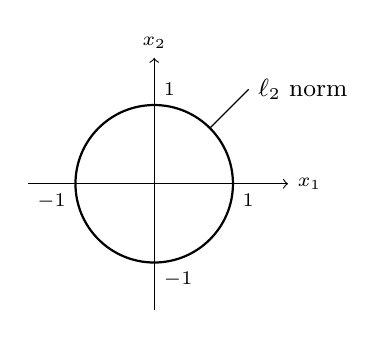
\begin{tikzpicture}[scale=1.0]
\draw[->] (-1.6,0) -- (1.7,0) node[right] {\scriptsize$x_1$};
\draw[->] (0,-1.6) -- (0,1.6) node[above] {\scriptsize$x_2$};
\draw[thick] (0,0) circle (1);
\node[below left] at (-1,0) {\scriptsize$-1$};
\node[below right] at (1,0) {\scriptsize$1$};
\node[above right] at (0,1) {\scriptsize$1$};
\node[below right] at (0,-1) {\scriptsize$-1$};
\draw (0.707,0.707) -- (1.2,1.2) node[right] {\small$\ell_2$ norm};
\end{tikzpicture}
\qquad\qquad
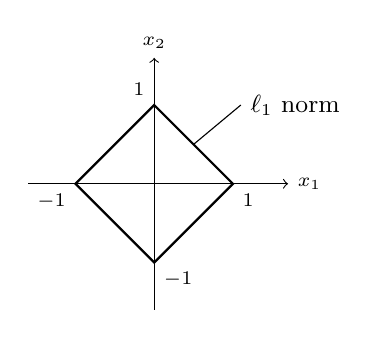
\begin{tikzpicture}[scale=1.0]
\draw[->] (-1.6,0) -- (1.7,0) node[right] {\scriptsize$x_1$};
\draw[->] (0,-1.6) -- (0,1.6) node[above] {\scriptsize$x_2$};
\draw[thick] (1,0) -- (0,1) -- (-1,0) -- (0,-1) -- cycle;
\node[below left] at (-1,0) {\scriptsize$-1$};
\node[below right] at (1,0) {\scriptsize$1$};
\node[above left] at (0,1) {\scriptsize$1$};
\node[below right] at (0,-1) {\scriptsize$-1$};
\draw (0.5,0.5) -- (1.1,1.0) node[right] {\small$\ell_1$ norm};
\end{tikzpicture}
\end{center}
\end{example}

\paragraph{$\ell_p$ norm.} The \term{$\ell_p$ norm} is
\[
\norm{x}_p = \left(\sum_{i=1}^{n}\abs{x_i}^p\right)^{1/p} \quad\text{where } p\ge1
\]
\paragraph{$\ell_\infty$ norm.} The \term{$\ell_\infty$ norm} is
\[
\norm{x}_\infty = \max_i\abs{x_i} = \lim_{p\to\infty}\norm{x}_p
\]
\needspace{9\baselineskip}
For $\V=\R^2$: $x=(x_1,x_2)\T$, \ $\norm{x}_p = \left(\abs{x_1}^p+\abs{x_2}^p\right)^{1/p}$. For $x_1=2$ \& $x_2=3$:
\begin{align*}
\norm{\bmat{2\\3}}_p &= (2^p+3^p)^{1/p}\\
&= (3^p)^{1/p}\cdot\left(1+\left(\tfrac23\right)^p\right)^{1/p}\\
&= 3\left(1+\left(\tfrac23\right)^p\right)^{1/p}\\
\lim_{p\to\infty}\norm{\bmat{2\\3}}_p &= 3 = \max\left(\abs{x_1},\abs{x_2}\right) = \norm{\bmat{2\\3}}_\infty
\end{align*}
\explain{$\left(\tfrac23\right)^p\to0$, so the factor $\left(1+(\tfrac23)^p\right)^{1/p}\to1$. In general the largest $\abs{x_i}$ dominates the sum: $\max_i\abs{x_i}\le\norm{x}_p\le n^{1/p}\max_i\abs{x_i}$ and $n^{1/p}\to1$.}

\sep
$\blacktriangleright$ Unit spheres $\norm{x}_p=1$, i.e.\ $\norm{x-0_{\V}}_p=1$. The $\ell_\infty$ unit sphere is $\max(\abs{x_1},\abs{x_2}) = 1$.
\begin{center}
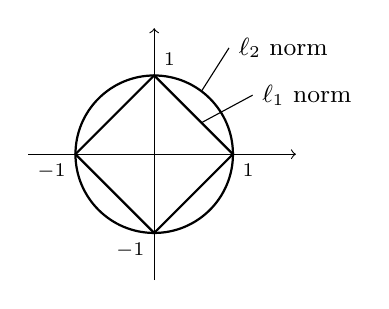
\begin{tikzpicture}[scale=1.0]
\draw[->] (-1.6,0) -- (1.8,0);
\draw[->] (0,-1.6) -- (0,1.6);
\draw[thick] (0,0) circle (1);
\draw[thick] (1,0) -- (0,1) -- (-1,0) -- (0,-1) -- cycle;
\node[below left] at (-1,0) {\scriptsize$-1$};
\node[below right] at (1,0) {\scriptsize$1$};
\node[above right] at (0,1) {\scriptsize$1$};
\node[below left] at (0,-1) {\scriptsize$-1$};
\draw (0.6,0.8) -- (0.95,1.35) node[right] {\small$\ell_2$ norm};
\draw (0.6,0.4) -- (1.25,0.75) node[right] {\small$\ell_1$ norm};
\end{tikzpicture}
\qquad\qquad
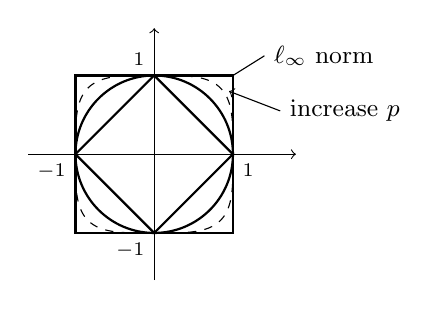
\begin{tikzpicture}[scale=1.0]
\draw[->] (-1.6,0) -- (1.8,0);
\draw[->] (0,-1.6) -- (0,1.6);
\draw[thick] (-1,-1) rectangle (1,1);
\draw[thick] (0,0) circle (1);
\draw[thick] (1,0) -- (0,1) -- (-1,0) -- (0,-1) -- cycle;
% intermediate p (p = 4): |x1|^4 + |x2|^4 = 1
\draw[dashed,domain=0:360,samples=145,smooth,variable=\t]
  plot ({sign(cos(\t))*abs(cos(\t))^(0.5)},{sign(sin(\t))*abs(sin(\t))^(0.5)});
\node[below left] at (-1,0) {\scriptsize$-1$};
\node[below right] at (1,0) {\scriptsize$1$};
\node[above left] at (0,1) {\scriptsize$1$};
\node[below left] at (0,-1) {\scriptsize$-1$};
\draw (1,1) -- (1.4,1.25) node[right] {\small$\ell_\infty$ norm};
\draw[->] (1.6,0.55) node[right] {\small increase $p$} -- (0.95,0.8);
\end{tikzpicture}
\end{center}
\explain{Dashed curve: $\abs{x_1}^p+\abs{x_2}^p=1$ for an intermediate $p$ (drawn for $p=4$); as $p$ increases the unit sphere moves from the $\ell_2$ circle towards the $\ell_\infty$ square.}

\sep
For $p=1/2$:
\[
\norm{x}_{1/2} = \left(\abs{x_1}^{1/2}+\abs{x_2}^{1/2}\right)^2
\]
\explain{It satisfies (N1) \& (N2) but need not satisfy the triangle inequality (N3).}
Counterexample:
\[
x=\bmat{9\\0}, \quad y=\bmat{0\\4}, \quad x+y=\bmat{9\\4}
\]
\begin{align*}
\norm{x+y}_{1/2} &= \left(\sqrt9+\sqrt4\right)^2 = 25\\
\norm{x}_{1/2}&=9, \qquad \norm{y}_{1/2}=4\\
\norm{x+y}_{1/2} &\not\le \norm{x}_{1/2}+\norm{y}_{1/2}
\end{align*}
\[ \key{$p<1 \ \Rightarrow\ \text{no norms!}$} \]
\explain{Here $25>9+4=13$. Geometrically, for $p<1$ the ``unit sphere'' $\abs{x_1}^p+\abs{x_2}^p=1$ is star-shaped (curved inwards) and the unit ball is not convex; \key{a norm's unit ball is always convex}.}

% ===== Page 12 =====
\subsection{Norms on Function Spaces}\label{ss:function-norms}
\begin{center}\origpage{12}
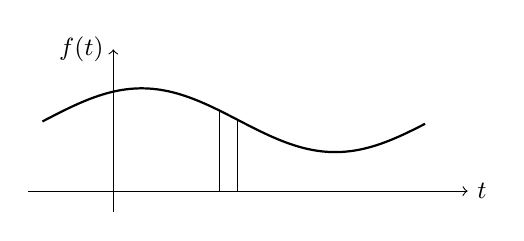
\begin{tikzpicture}[scale=0.9]
\draw[->] (-1.2,0) -- (5,0) node[right] {\small$t$};
\draw[->] (0,-0.3) -- (0,2) node[left] {\small$f(t)$};
\draw[thick,smooth,domain=-1:4.4,samples=60] plot (\x,{1.0+0.45*cos(deg(1.15*(\x-0.4)))});
% thin strip under the curve
\draw (1.5,0) -- (1.5,{1.0+0.45*cos(deg(1.15*1.1))});
\draw (1.75,0) -- (1.75,{1.0+0.45*cos(deg(1.15*1.35))});
\end{tikzpicture}
\end{center}
\[
\mathcal{L}_p = \left\{ f(\cdot) \;\middle|\; f:\R\to\R \text{ such that } \int_{-\infty}^{\infty}\abs{f(t)}^p\,dt<\infty \right\}, \qquad 1\le p<\infty
\]
\needspace{10\baselineskip}
\begin{align*}
\norm{f(t)}_p &= \left(\int_{-\infty}^{\infty}\abs{f(t)}^p\,dt\right)^{1/p} && \mathcal{L}_p \text{ norm}\\
\norm{f(t)}_1 &= \int_{-\infty}^{\infty}\abs{f(t)}\,dt && \mathcal{L}_1 \text{ norm}\\
\norm{f(t)}_2 &= \left(\int_{-\infty}^{\infty}\abs{f(t)}^2\,dt\right)^{1/2} && \mathcal{L}_2 \text{ norm}\\
\norm{f(t)}_\infty &= \sup_t\abs{f(t)} && \mathcal{L}_\infty \text{ norm}
\end{align*}
% corrected: notes had the L_p and L_2 integrals without dt, the L_1 norm without subscript, and max_t |f(t)| for L_infinity; the example below shows why sup is needed
\explain{These are the continuous analogues of the $\ell_p$ norms: the sum over $i$ becomes an integral over $t$.}

\sep
\needspace{12\baselineskip}
\begin{center}
$f(t) = 1-e^{-t},\quad t\ge0$
\qquad
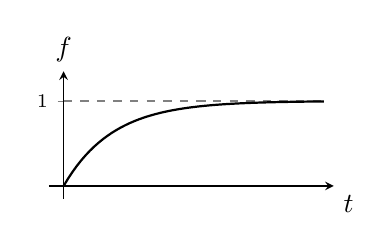
\begin{tikzpicture}[baseline=0.4cm]
\begin{axis}[width=5.2cm,height=3.2cm,axis lines=middle,xmin=-0.3,xmax=5.5,ymin=-0.15,ymax=1.35,
  xtick=\empty,ytick={1},xlabel={$t$},ylabel={$f$},
  xlabel style={anchor=north west},ylabel style={anchor=south},tick label style={font=\scriptsize}]
\addplot[dashed,gray,domain=0:5.3] {1};
\addplot[thick,domain=0:5.3,samples=60] {1-exp(-x)};
\end{axis}
\end{tikzpicture}
\end{center}
\explain{Value 1 is never reached. A maximum would have to be attained at a finite $t$, so $\max_t\abs{f(t)}$ does not exist here.}
The supremum, however, does exist:
\[ \sup_t\abs{f(t)} = 1 \quad (\text{least upper bound}) \]
\explain{Therefore \key{$\norm{f}_\infty$ is defined with $\sup$} (it always exists for bounded $f$), which equals $\max$ whenever the maximum is attained.}

\sep
\key{Integral norms do not satisfy $\norm{x}=0 \iff x=0_{\V}$!}
\begin{center}
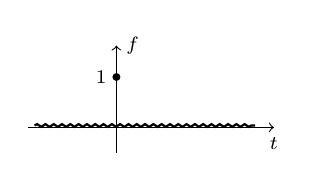
\begin{tikzpicture}[scale=0.8,baseline=0.2cm]
\draw[->] (-1.4,0) -- (2.5,0) node[below] {\scriptsize$t$};
\draw[->] (0,-0.4) -- (0,1.3) node[right] {\scriptsize$f$};
\fill (0,0.8) circle (1.8pt);
\node[left] at (0,0.8) {\scriptsize1};
\draw[thick,decorate,decoration={snake,amplitude=0.5pt,segment length=3pt}] (-1.3,0.03) -- (2.2,0.03);
\end{tikzpicture}
\qquad
$f(t) = \begin{cases} 1, & t=0\\ 0, & \text{otherwise}\end{cases}
\qquad\Rightarrow\qquad
\displaystyle\int_{-\infty}^{\infty}\abs{f(t)}\,dt = 0$
\end{center}
\explain{Such functions are equivalent to the zero function, as they take nonzero values only at finitely many points.}
\begin{insight}[How this is fixed]
$f\neq0$ but $\norm{f}_1=0$, so property (N1) fails on the set of all functions. The standard remedy: regard two functions as \emph{equal} in $\mathcal{L}_p$ if they differ only on a set of zero length (e.g.\ finitely many points), i.e.\ if $\norm{f-g}_p=0$. With this identification $\norm{\cdot}_p$ is a genuine norm on $\mathcal{L}_p$ for $p\ge1$ (the triangle inequality is Minkowski's inequality).
\end{insight}

\subsection{Matrix Norms}\label{ss:matrix-norms}
\[ A = \bmat{1&-2\\3&4}, \qquad \norm{A}=\,? \]

\subsubsection{Entrywise Norms (Frobenius)}
\needspace{14\baselineskip}
\paragraph{1st method.}
\[
\operatorname{Vec}(A) \triangleq \bmat{1\\3\\-2\\4}, \qquad A = \bmat{a_{11}&a_{12}\\a_{21}&a_{22}}
\]
\begin{align*}
\norm{A}_p = \norm{\operatorname{Vec}(A)}_p = \norm{\bmat{1\\3\\-2\\4}}_p &= \left(\abs{1}^p+\abs{3}^p+\abs{-2}^p+\abs{4}^p\right)^{1/p}\\
&= \left(\sum_{i,j}\abs{a_{ij}}^p\right)^{1/p}, \qquad p\ge1
\end{align*}
\begin{insight}[Numbers for this $A$]
\[
\norm{A}_1 = 1+2+3+4 = 10, \quad
\norm{A}_2 = \sqrt{1+4+9+16}=\sqrt{30}\approx5.48, \quad
\norm{A}_\infty = \max_{i,j}\abs{a_{ij}} = 4
\]
The case $p=2$ is the \term{Frobenius norm} $\norm{A}_F$. Since $\R^{m\times n}$ is a vector space that is identified with $\R^{mn}$ through $\operatorname{Vec}$, every vector norm gives a matrix norm in this way.
\end{insight}
